\begin{frame}{Bagging, Random Forests, Boosting, and Bayesian Additive Regression Trees}
\begin{itemize}

    \item We'll begin with define an \textit{ensemble method}. \pause 
    
    \item An ensemble method is an approach that combines many simple \textit{building ensemble block} models to obtain a single and potentially very powerful model. \pause 
    \item These simple building block models are sometimes known as \textit{weak learners}, since they may lead to mediocre predictions on their own. \pause 

    \item We will now discuss bagging, random forests, boosting, and Bayesian learners additive regression trees. \pause 
    
    \item These are ensemble methods for which the simple building block is a regression or a classification tree. 
\end{itemize}


\end{frame}

\subsection{Bagging}
\begin{frame}{Bagging}
    \begin{itemize}
        \item Recall that given a set of $n$ independent observations $Z_1 , \cdots , Z_n$ , each with $Var(Z_i) = \sigma^2$, then $Var(\bar{Z}) = \sigma^2/n$. \pause \\ 
        $\rightarrow$ \textcolor{blue}{Averaging a set of observations reduces variance}.\pause 

        \item We use this idea to do resampling with replacement (bootstrap sample) for the training dataset. \pause 

  \end{itemize}
\end{frame}



\begin{frame}{Bagging}

\footnotesize

\begin{columns}[T]

\column{0.5\linewidth}

        \textbf{For regression:} \\ \pause 
        \begin{itemize}
            \item We generate $B$ different bootstrapped training sets. \pause
            \item Train the model on the $b$th bootstrapped training set % in order to get $\hat{f}^{*b}(x)$. \pause 
            \item  Average all the predictions. \pause 
%        \begin{equation*}
%            \hat{f}_{bag}(x) = \frac{1}{B} \sum_{b=1}^B \hat{f}^{*b}(x).
%        \end{equation*} \pause 

        \end{itemize}
    
        \begin{figure}
            \centering
            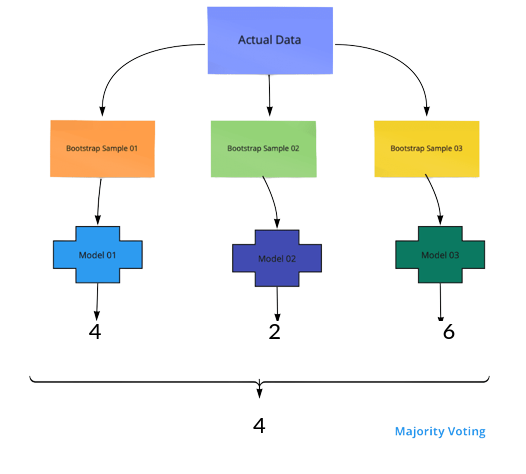
\includegraphics[height=4cm]{bagging-boosting/bagging-regress.png}
        \end{figure} \pause 

\column{0.5\linewidth}


    \textbf{For classification}:\\ \pause 

    \begin{itemize}
        \item We generate $B$ different bootstrapped training sets. \pause
        \item Record the class predicted by each of the $B$ trees.  \pause
        \item Take the \textit{majority vote} as the prediction. \pause
    \end{itemize}

     \begin{figure}
            \centering
            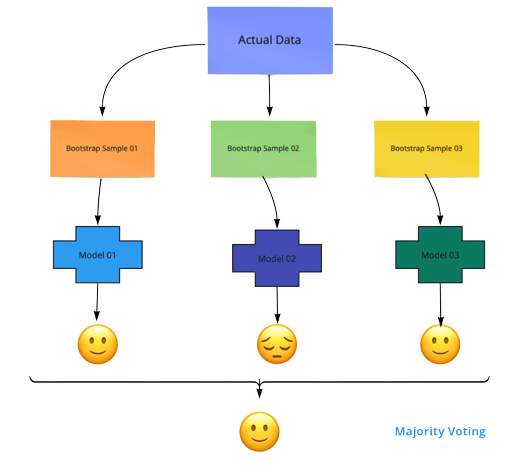
\includegraphics[height=4cm]{bagging-boosting/bagging-class.png}
    \end{figure} 
    

    
\end{columns}


\end{frame}


\begin{frame}{Bagging}{Out-of-Bag Error Estimation}

    \begin{itemize}
        \item On average, each bagged tree makes use of around $2/3$ of the observations. \pause 
        \item The remaining $1/3$ of the observations not used to fit a given bagged tree are referred to as the \textbf{out-of-bag (OOB) observations}. \pause 
        \item We can predict the response for the $i$th observation using each of the trees in which that observation was OOB.  \pause 
        \item The final prediction is then the average predicted responses (for regression) or the majority vote (for classification). \pause 
        \item This leads to a single OOB prediction for the $i$th observation. \pause 
        \item The resulting OOB error is a valid estimate of the test error for the bagged model. 
        
    \end{itemize}

    
\end{frame}

\begin{frame}{Bagging}{Out-of-Bag Error Estimation}

\begin{figure}
    \centering
    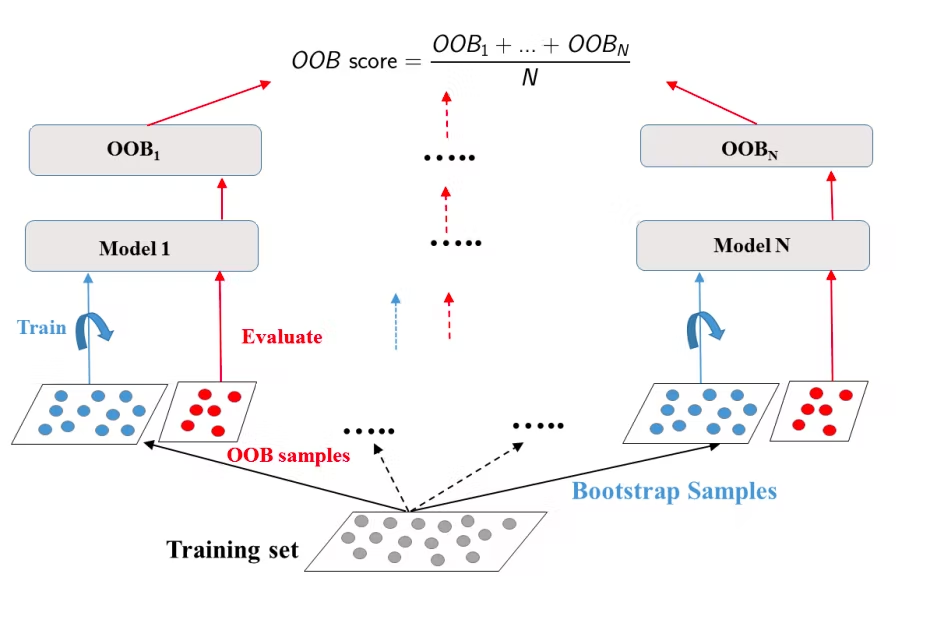
\includegraphics[height=7cm]{bagging-boosting/oob.png}
\end{figure}
    
\end{frame}

\begin{frame}{Bagging}{Variable importance measures}

One can obtain an overall summary of the importance of each predictor.  \pause 

\begin{columns}[T]

\column{0.5\linewidth}

        \textbf{For regression:} \\ \pause 
        \begin{itemize}

        \item We record the total amount that the $RSS$ is decreased due to splits over a given predictor, averaged over all $B$ trees. \pause 
        
        \item A large value indicates an important predictor. \pause 

        \end{itemize}
    
 

\column{0.5\linewidth}


    \textbf{For classification}:\\ \pause 

    \begin{itemize}

    \item We add up the total amount that the Gini index is decreased by splits over a given predictor, averaged over all $B$ trees. \pause 

    \item A small value indicates an important predictor.

    \end{itemize}

 
    
\end{columns}

    
\end{frame}

\subsection{Random forests}
\begin{frame}{Random Forests}
    \begin{itemize}
        \item As in bagging, we build a number of decision trees on bootstrapped samples. \pause 

        \item But here, a random sample of $m$ predictors is chosen as split candidates from the full set of $p$ predictors. \pause

        \item Typically we choose $m \approx \sqrt{p}$ \pause 
    \end{itemize}

    \textbf{Why?} \pause 

    \begin{itemize}
    \item Suppose that there is one strong predictor in the data set, along with others moderately strong predictors. \pause 

    \item In the collection of bagged trees, most or all of the trees will use this strong predictor in the top split. \pause 

    \item Consequently, all of the bagged trees will look quite similar to each other. \pause 

    \item Then the predictions will be highly correlated. \pause 
\end{itemize}


\textbf{The solution} \pause 

    \begin{itemize}
        \item Random forests overcome this problem by forcing each split to consider only a subset of the predictors. \pause 
        
        \item On average $(p - m)/p$ of the splits will not even consider the strong predictor, and so other predictors will have more of a chance.
    \end{itemize}
    

    
\end{frame}

\subsection{Boosting}
\begin{frame}{Boosting}

\begin{itemize}
    \item Boosting refers to an ensemble method in which many predictors are trained and each predictor learns from the errors of its predecessor. \pause 

    \item  More formally, in boosting many \textbf{weak learners} are combined to form a \textbf{strong learner}. \pause

    $\rightarrow$A weak learner is a model doing slightly better than random guessing.  \pause 

    \item Here, an ensemble of predictors are trained \textit{sequentially} and each predictor tries to correct the errors made by its predecessor. \pause 
    \item Boosting has three tuning parameters:

    \begin{enumerate}
        \item \textbf{The number of trees $B$}: selected by cross-validation. \pause 

        \item \textbf{The shrinkage parameter $\eta$}: this controls the rate at which boosting learns. \pause 

        \item \textbf{The number $d$ of splits in each tree}: which controls the complexity of the boosted ensemble.
    \end{enumerate}

    
\end{itemize}
    
\end{frame}

\begin{frame}{Boosting}
\begin{figure}
    \centering
    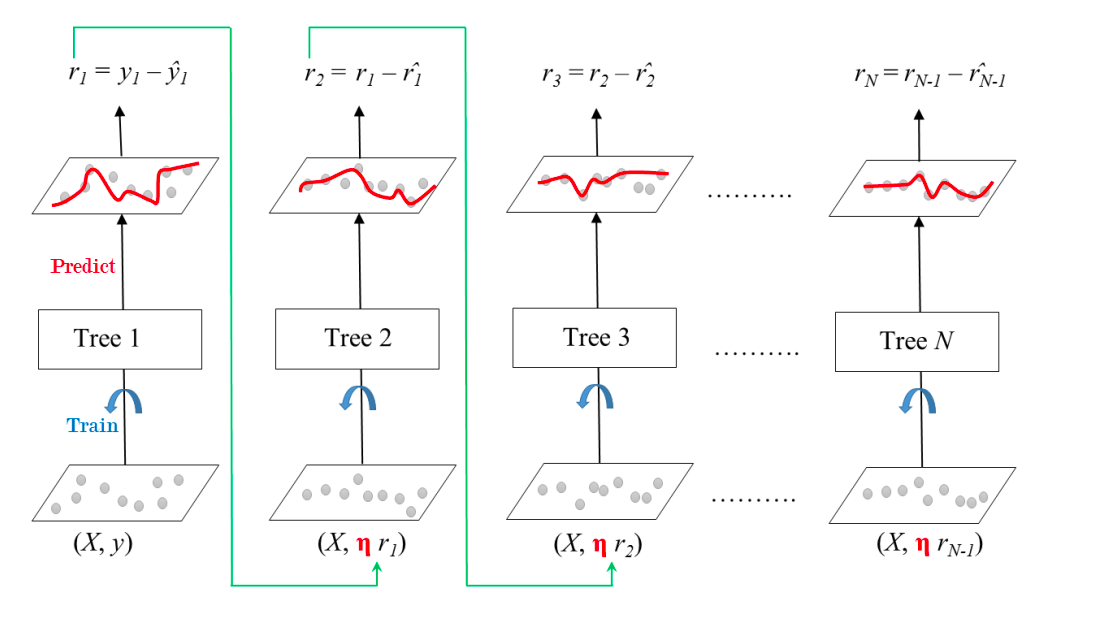
\includegraphics[height=6cm]{bagging-boosting/boosting.png}
\end{figure}
    
\end{frame}

\subsection{Bayesian Additive Regression Trees}
\begin{frame}{Bayesian Additive Regression Trees (BART)}

BART is related to both approaches seen before: \pause 
\begin{itemize}
    \item Each tree is constructed in a random manner. \pause 

    \item Each tree tries to capture signal not yet accounted for by the current model. \pause 

    \item The main novelty in BART is the way in which new trees are generated. \pause 
\end{itemize}


But first, some notation: \pause 

\begin{itemize}
    \item Let $K$ denote the number of regression trees. \pause 

    \item $B$ is the number of iterations for which the BART algorithm will be run. \pause 

    \item $\hat{f}_k^b(x)$ is the prediction at $x$ for the $k$th regression tree used in the $b$th iteration. \pause 

    \item At the end of each iteration, all the $K$ trees from $b$ will be summed, 

    \begin{equation*}
        \hat{f}^b(x) = \sum_{k=1}^K \hat{f}_k^b(x) \text{ for } b= 1, \ctods , B. 
    \end{equation*}
\end{itemize}

    
\end{frame}

\begin{frame}{Bayesian Additive Regression Trees (BART)}
    The algorithm is described as follows, \pause 

    \begin{enumerate}
        \item Initialized all trees to have a single root node, with a prediction given by, \pause 

        \begin{equation*}
            \hat{f}_k^1(x) = \frac{1}{nK} \sum_{i=1}^n y_i.
        \end{equation*} \pause 

        \item Compute the prediction in for all the $K$ trees as,  \pause 

        \begin{equation*}
            \hat{f}^1(x) = \frac{1}{n} \sum_{i=1}^n y_i.
        \end{equation*} \pause 

        \item Update each of the $K$ trees in each iteration. \\ \pause 
        For $b = 2, \cdots, B:$  \pause 
        \begin{enumerate}[a]
            \item For $k = 1, \cdots , K$: compute the \textbf{current partial residual}, \pause 
            \begin{equation*}
                r_i = y_i - \sum_{k' < k} \hat{f}_{k'}^b (x_i) - \sum_{k'>k} \hat{f}^{b-1}_{k'}(x_i) \, \, i = 1, \cdots, n.
            \end{equation*} \pause 
            \item Fit a new tree $\hat{f}_{k'}^b (x_i)$ with $r_i$, by randomly perturbing $\hat{f}^{b-1}_{k'}(x_i)$. \pause 
            \item Compute $\hat{f}_{k}^b (x_i)$. 
        \end{enumerate}
            
    \end{enumerate}
    
\end{frame}

\begin{frame}{Bayesian Additive Regression Trees (BART)}

\begin{enumerate}
    \setcounter{enumi}{4}
    \item Typically  models obtained in the earlier iterations — known as the \textbf{burn-in} period— tend not to provide very good results. So we throw away the $L$ burn-in iterations and to obtain a single prediction, we compute: \pause 

    \begin{equation*}
        \hat{f}(x) = \frac{1}{B-L} \sum_{b=L+1}^B \hat{f}^b(x). 
    \end{equation*} \pause 
    
\end{enumerate}

\textbf{What is the random perturbation?} \pause 

\begin{enumerate}
    \item We may change the structure of the tree by adding or pruning branches. \pause 

    \item We may change the prediction in each terminal node of the tree. 
\end{enumerate}

    
\end{frame}

\begin{frame}{Bayesian Additive Regression Trees (BART)}

\begin{figure}
    \centering
    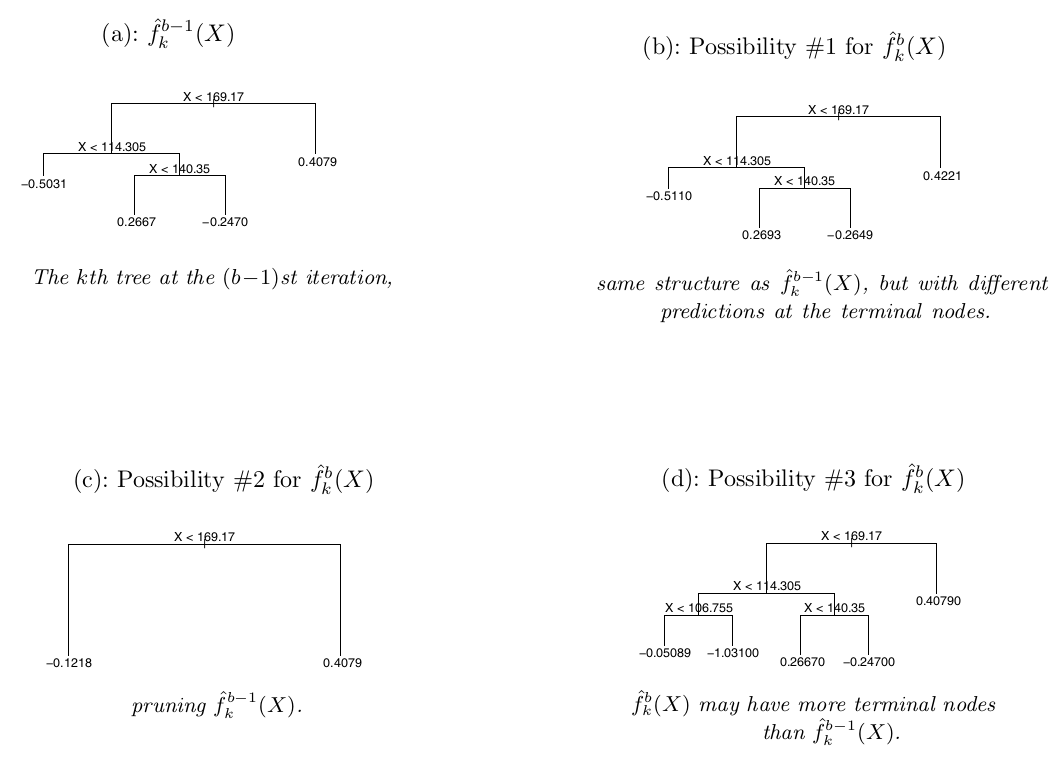
\includegraphics[height=7cm]{bagging-boosting/barts-random.png}
    
\end{figure}
    
\end{frame}

\subsection{Summary}
\begin{frame}{Summary}
\begin{itemize}
    \item The idea of this ensemble methods is to use many \textit{weak learners} to construct a \textit{strong learner}. \pause 

    \item They have the flexibility and the ability to handle predictors of mixed types. \pause 

    \item We have now seen four approaches for fitting an ensemble of trees:

    \begin{enumerate}
        \item \textbf{Bagging}: the trees are grown independently on \textit{random samples} of the observations and the trees tend to be quite similar to each other. \pause 

        \item \textbf{Random forests}: overcomes the problem with \textit{bagging} by using a \textit{random subset} of the features on each split. \pause 

        \item \textbf{Boosting}: we do not draw any random samples, and each new tree is fit to the signal that is left over from the earlier trees. \pause 

        \item \textbf{BART}: we once again only make use of the original data, and we grow the trees successively. However, each tree is perturbed. 
    \end{enumerate}

\end{itemize}
    
\end{frame}